\documentclass[a4paper,12pt]{article}
\usepackage[utf8]{inputenc}
\usepackage[T1]{fontenc}
\usepackage{amsmath}
\usepackage{graphicx}
\usepackage{geometry}
\geometry{margin=1in}
\usepackage{float}
\usepackage{float}

\title{Solving the Single-Source Unsplittable Flow Problem with Metaheuristic Approaches}
\author{\\Aleksa Toroman 84/2018 \\\\ Univerzitet u Beogradu, Matematički fakultet}
\date{\today}

\begin{document}

\maketitle

\newpage
\renewcommand{\contentsname}{Table of contents}
\tableofcontents

\newpage

\section{Introduction}

The Single-Source Unsplittable Flow Problem (SSUFP) is a well-known problem in network flow optimization. Given a graph $G = (V, E)$ with a source vertex $s$ and a collection of sinks $t_1, \ldots, t_k$ associated with integer demands $\rho_1, \ldots, \rho_k$, the goal is to route a single flow path from the source $s$ to each sink $t_i$ such that the total flow across any edge $e \in E$ does not exceed the edge’s capacity $c(e)$. Formally, the objective is to minimize the maximum ratio $\frac{f(e)}{c(e)}$ over all edges, where $f(e)$ is the total flow routed across edge $e$.

\noindent \textbf{Problem Statement:}

\begin{itemize}
    \item \textbf{Instance:} A directed graph $G=(V, E)$ with edge capacities $c: E \to \mathbb{Z}^+$, a source node $s$, and $k$ sinks $t_1, \ldots, t_k$, each with a demand $\rho_i$. Each demand $\rho_i$ must be routed along a single path from $s$ to $t_i$. Additionally, each vertex can have any number of sinks.
    \item \textbf{Objective:} Route each demand in such a way that the total flow routed across any edge $e \in E$ is bounded by its capacity, $c(e)$.
    \item \textbf{Measure:} Minimize the maximum congestion, defined as $\max_{e \in E} \frac{f(e)}{c(e)}$.
\end{itemize}

\noindent The SSUFP is an NP-hard problem, meaning that there is no known polynomial-time algorithm that can solve all instances optimally. The difficulty of the problem lies in the fact that flows cannot be split across multiple paths for each demand; every demand must be routed along a single path. This constraint introduces significant challenges in finding feasible flow paths, especially as the number of demands or the size of the network increases. \\

\noindent \textbf{Example Problem:} Consider a graph $G$ with 5 nodes and 6 edges, where node $s$ is the source and nodes $t_1, t_2$, and $t_3$ are the sinks. Each edge has a capacity $c(e)$, and each sink has an associated demand $\rho_i$. An example solution would route each demand along a single path, while ensuring that no edge capacity is exceeded. (An illustrative figure and result will be placed here.)

\noindent \textbf{Complexity and Challenges:}

\

\noindent The Single-Source Unsplittable Flow Problem is known to be NP-hard, which implies that it is computationally intractable to find the exact solution for large instances. The primary challenge arises from the unsplittable nature of the flow, meaning that each demand must be routed along a single path. This requirement limits the flexibility in distributing the flow and leads to congestion on certain edges, which increases the difficulty of finding feasible solutions.
\\

\noindent Several factors increase the complexity of the problem:

\begin{itemize}
    \item \textbf{Edge Congestion:} Ensuring that no edge exceeds its capacity is challenging when multiple demands compete for the same edges.
    \item \textbf{Path Selection:} Selecting the right paths for each demand is crucial to avoid overloading the network.
    \item \textbf{Scalability:} As the number of demands or the size of the network increases, the number of possible path combinations grows exponentially, making the problem harder to solve.
\end{itemize}

\noindent \textbf{Known Algorithms:}

\

\noindent Despite the complexity, there are approximation algorithms available that provide good solutions in practice. Some notable results include:
\begin{itemize}
    \item A 2-approximation algorithm for minimizing congestion exists when certain conditions are met, meaning that the algorithm can find a solution with at most twice the optimal congestion.
    \item The problem is approximable within a factor of 3.23 for directed graphs, which provides a performance guarantee on how far the solution is from the optimal.
    \item It is also known that no approximation algorithm can achieve a performance better than \( \frac{3}{2} - \epsilon \) for any $\epsilon > 0$, demonstrating the inherent difficulty of the problem.
\end{itemize}

\noindent In addition to these approximation algorithms, metaheuristic approaches such as Simulated Annealing, Genetic Algorithms, and Variable Neighborhood Search offer heuristic methods to find near-optimal solutions. These algorithms are particularly useful for large instances where exact methods become impractical.

\

\noindent The remainder of this report will explore metaheuristic approaches to solving the SSUFP, focusing on their implementation and the quality of the solutions they provide.

\section{Research Methodology}

The research for solving the Single-Source Unsplittable Flow Problem (SSUFP) was conducted in several stages, each contributing to the overall understanding and development of a practical solution. The following steps outline the methodology used in this project:

\begin{enumerate}
    \item Getting familiar with the problem and reading existing literature.
    \item Creating a custom graph textual representation.
    \item Developing a graph generation library for instance creation.
    \item Building core infrastructure classes in Python, including representations for the graph, demands, and utilities.
    \item Implementing algorithms, including Brute Force, Simulated Annealing, and Genetic Algorithm.
    \item Analyzing and evaluating the results of the implementations.
\end{enumerate}

Each of these steps will be elaborated in the subsequent sections.

\subsection{Getting Familiar with the Problem and Literature Review}

The initial phase of the project involved gaining a comprehensive understanding of the Single-Source Unsplittable Flow Problem (SSUFP). This included studying the problem's mathematical formulation, exploring related optimization challenges, and reviewing existing literature on approximation algorithms. Research papers on unsplittable flow problems and related NP-hard network optimization problems provided valuable insights into the complexities and potential solution techniques.

\subsection{Creating a Custom Graph Textual Representation}

To represent the input graph for the Single-Source Unsplittable Flow Problem, a custom textual format was designed. This format is easy to parse and process programmatically, and it captures all necessary details, including vertices, edges, capacities, and demands for each sink.

The structure of the graph representation is as follows:
\begin{itemize}
    \item The first line contains the number of vertices.
    \item The second line indicates the number of edges.
    \item The third line identifies the source vertex.
    \item The next \(N\) lines represent each edge in the format: \textit{source vertex, destination vertex, capacity}, where the graph is directed.
    \item After the edges, there is a line containing the number of sink vertices.
    \item The remaining lines correspond to the sink vertices, where each line contains the index of the vertex, the number of sinks that vertex has, and their respective demands.
\end{itemize}

\noindent \textbf{Example Representation:}

\begin{verbatim}
5
7
1
1 2 7
1 3 3
2 4 6
2 3 5
2 5 4
5 4 2
1 5 5
2
4 1 3
3 2 2 1
\end{verbatim}

\noindent In this example:
\begin{itemize}
    \item The graph has 5 vertices and 7 edges.
    \item Vertex 1 is the source.
    \item The edges are represented as directed connections between vertices, with specified capacities.
    \item There are 2 sink vertices, with vertex 3 having two demands (2 and 1), and vertex 4 having one demand (3).
\end{itemize}

\begin{figure}[H]
\centering
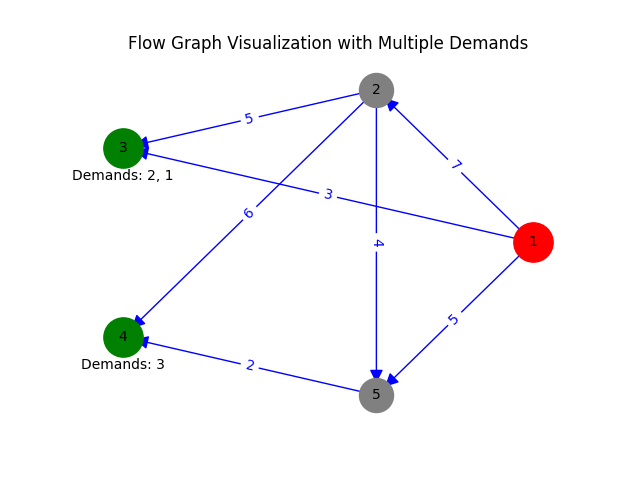
\includegraphics[width=100mm]{graph-1.png}
\caption{Example graph problem instance}
\label{fig:graph_example}
\end{figure}

\subsection{Graph Generation Library for Instance Creation}

In order to effectively test the algorithms, a graph generation library was developed due to the lack of a pre-existing dataset for the Single-Source Unsplittable Flow Problem (SSUFP). Initially, I created a few simple examples that could be manually calculated, serving as a basic test for the algorithms. However, for larger-scale testing and analysis, I implemented a mechanism to generate random graph instances of various sizes.

\

\noindent The graph generation uses the NetworkX library in python to create directed random graphs, with adjustments made to tailor the graphs specifically for the SSUFP problem. The process involves the following key steps:

\begin{itemize}
    \item Initial Graph Generation: A random directed graph is generated using the Erdős-Rényi model, with an edge probability that varies depending on the graph size. For small graphs, the edge probability is 0.2, for medium graphs it is 0.15, and for large graphs it is 0.1. These probabilities influence the density of edges in the generated graph.
    
    \item Graph Adjustments: After generating the random graph, certain adjustments are made:
    \begin{itemize}
        \item Outgoing edges from non-source vertices to the source are removed to avoid reverse flow.
        \item Outgoing edges from sink vertices are removed to ensure sinks do not act as intermediate vertices for other flows.
        \item If no path exists between the source and any sink, random "hops" are added between intermediate nodes to create a valid path, ensuring at least one solution exists for each instance.
    \end{itemize}
    
    \item Edge Capacities: Capacities for the edges are assigned randomly within a range of 10 to 40. These capacities represent the maximum flow that each edge can carry.
    
    \item Demand Generation: Demands for sink vertices are generated based on the type of graph. For balanced graphs, each sink vertex typically has 1 or 2 demands, while for large-demand graphs, each sink can have up to 3 demands. The demand values are random integers, but they are kept small compared to the edge capacities to ensure feasible solutions.
    
    \item Graph Sizes:
    \begin{itemize}
        \item Small Graphs: Small instances contain between 5 and 10 nodes, with 1 to 3 demands.
        \item Medium Graphs: Medium instances range from 15 to 25 nodes, with 3 to 6 demands.
        \item Large Graphs: Large instances contain between 30 and 50 nodes, with 5 to 10 demands.
    \end{itemize}
    
    \item Graph Serialization: After generating and adjusting the graph, it is serialized into a given text format described earlier. The serialization includes all nodes, edges, capacities, and demands. The generated graph is saved as a text file, where each graph's filename includes a hash for uniqueness.
    
\end{itemize}

\noindent The graph generation library enables the creation of instances with varying complexities, which are crucial for testing and evaluating the performance of the implemented algorithms. Below is a graphical illustration of a randomly generated graph instance (image will be inserted here):

\subsection{Building Core Infrastructure Classes in Python}

To effectively implement and test various algorithms for solving the Single-Source Unsplittable Flow Problem (SSUFP), several core infrastructure components were developed in Python. These include essential classes to represent the graph, demands, and results, as well as utility functions used by the algorithms. The code was designed to be modular and reusable, supporting various hyperparameter configurations and testing scenarios.

\noindent \textbf{Core Classes:}
\begin{itemize}
    \item \textbf{Graph Class}: This class represents the underlying network with nodes and edges, storing relevant information such as capacities and connections between vertices as well as list of demands.
    \item \textbf{Demand Class}: Each demand corresponds to a specific sink vertex and its associated demand value, ensuring that the each demand in graph must be routed unsplittably along a single path.
    \item \textbf{Result Class}: This class holds the results of each algorithm run, tracking information such as the time taken, whether the solution was feasible, and the objective function value.
\end{itemize}

\noindent \textbf{Utility Functions:}
In addition to the core classes, several utility functions were implemented to assist the algorithms:
\begin{itemize}
    \item \textbf{Feasibility Check}: A utility function checks whether a solution is feasible by verifying that the flow on each edge does not exceed its capacity. This operation is of polynomial time complexity.
    \item \textbf{Random Path Finder}: A depth-first search (DFS) based function is used to find random paths between two nodes. This function is especially useful in metaheuristic algorithms like Simulated Annealing and Genetic Algorithms to explore different routing paths.
\end{itemize}

\noindent \textbf{Hyperparameter Support:}
The infrastructure is flexible enough to allow passing different hyperparameters to various algorithms. Similar to the grid search in libraries like \textit{scikit-learn}, different combinations of hyperparameters can be tested to optimize the performance of the algorithms. Parameters such as cooling rate for Simulated Annealing or population size for the Genetic Algorithm can be easily configured via command-line options.

\

\noindent \textbf{Automation and Result Logging:}
A root file structure was designed to automatically run different algorithms and store the results in a well-organized format. The results for each algorithm run are saved in CSV files, which include details such as:
\begin{itemize}
    \item Algorithm used
    \item Hyperparameters used
    \item Time taken by the algorithm
    \item Whether the solution was feasible
    \item Objective function value (optimization target)
\end{itemize}

\noindent This mechasnism also allows to store different artifacts such as different kinds of plots in well organized structure during the algorithm execution.

\

\noindent Additionally, a command-line interface allows users to specify which algorithms to run, and where is the root folder of given example instances. The results are automatically exported into an csv file in above mentioned file structure, making it easier to analyze and compare the performance of different algorithms across multiple instances.

Below is an example of the folder structure and a snippet from the result log:

\begin{figure}[H]
    \centering
    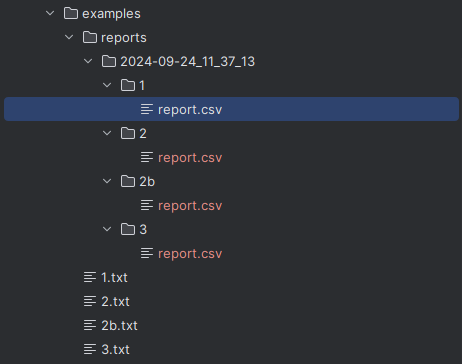
\includegraphics[width=0.5\textwidth]{reports-structure.png}
    \caption{Screenshot of result file structure and log}
\end{figure}

\begin{figure}[H]
    \centering
    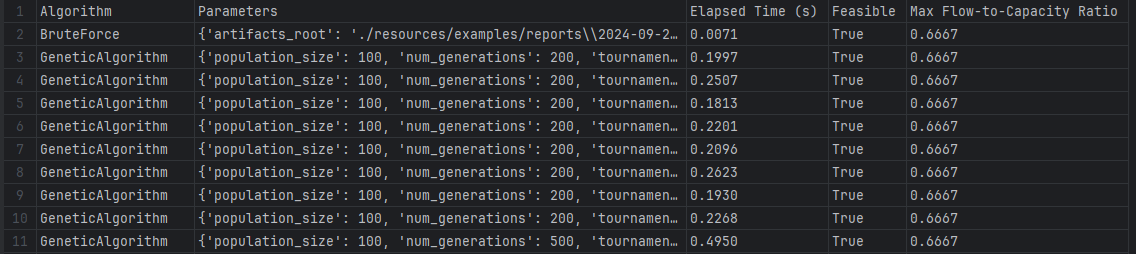
\includegraphics[width=0.5\textwidth]{report-snippet.png}
    \caption{Snippet of result log showing algorithm details and performance}
\end{figure}


\subsection{Algorithm Implementation}

To solve the Single-Source Unsplittable Flow Problem (SSUFP), several algorithms were implemented, each offering different approaches to finding feasible and near-optimal solutions. The algorithms developed include both exact and metaheuristic techniques:

\begin{itemize}
    \item \textbf{Brute Force}: A straightforward approach that explores all possible paths from the source to each sink and evaluates all combinations of paths to find the best feasible solution. Due to the problem's NP-hard nature, this method is only feasible for small instances.
    
    \item \textbf{Simulated Annealing}: A metaheuristic algorithm inspired by the annealing process in metallurgy. It starts with an initial solution and explores neighboring solutions, gradually reducing the likelihood of accepting worse solutions as the temperature decreases. This allows for exploration of the solution space while avoiding getting stuck in local optima.
    
    \item \textbf{Variable Neighborhood Search (VNS)}: This algorithm systematically changes the neighborhood structures during the search. By altering the neighborhood, VNS explores different parts of the solution space, switching between local searches to escape local optima and find better solutions.
    
    \item \textbf{Genetic Algorithm (GA)}: A population-based optimization algorithm that mimics natural selection. The algorithm generates an initial population of solutions and evolves them using operations like crossover and mutation. Over several generations, the population converges towards a feasible and near-optimal solution.
\end{itemize}

\noindent Each of these algorithms was implemented in Python, leveraging the core infrastructure classes and utility functions described earlier. The flexibility of the infrastructure allowed for easy experimentation with different hyperparameters for each algorithm, facilitating a detailed comparison of their performance.

\

\noindent  In the following sections, we will present the results obtained from each algorithm, how is it implemented, along with a comparison of their effectiveness, execution time, and quality of solutions.

\subsection{Brute Force Algorithm}

The Brute Force approach is a simple and exhaustive method used to solve the Single-Source Unsplittable Flow Problem (SSUFP). It retrieves all possible paths from the source to each sink vertex, including cases where sink vertices have multiple demands. Using the NetworkX library, which can efficiently find all simple paths between vertices, this process is straightforward for small graphs.

\noindent Once the paths are retrieved, the algorithm generates all combinations of possible routes using the Cartesian product of the paths for each demand. After generating the combinations, it checks each combination for feasibility by ensuring that the total flow on any edge does not exceed its capacity. For feasible solutions, the algorithm calculates the objective function, which is the maximum congestion over all edges.

\noindent While this approach works well for small graphs, it becomes computationally infeasible for even moderately complex graphs due to the exponential growth in the number of path combinations. This makes the Brute Force method unsuitable for larger instances.

\

\noindent \textbf{Example:}
In one example graph with 11 vertices and 3 sink nodes, where two of the sink nodes have two demands each, the number of possible paths for each demand is as follows:

\begin{verbatim}
Number of paths for each demand: [19, 19, 38, 38, 11]
\end{verbatim}

\noindent This results in a total of 5,734,124 combinations. Out of these, only 3,041 combinations were feasible. The Brute Force algorithm completed in 63.03 seconds for this instance.

\begin{figure}[H]
    \centering
    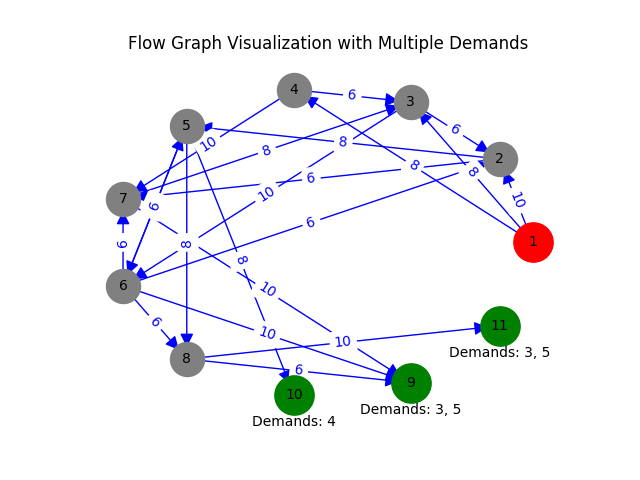
\includegraphics[width=0.5\textwidth]{brute-force-example.png}
    \caption{Example graph solved using brute force algorithm}
\end{figure}

\begin{itemize}
    \item Total combinations: 5,734,124
    \item Feasible combinations: 3,041
    \item Time taken: 63.03 seconds
\end{itemize}

\noindent  While Brute Force provides an exact solution, its time complexity grows exponentially, making it impractical for graphs with many paths and multiple demands. This highlights the need for more scalable, approximate methods like Simulated Annealing and Genetic Algorithms for larger instances.

\subsection{Results Analysis}

% Placeholder for results analysis
\end{document}


\end{document}
